\documentclass[12pt, a4paper]{report}
\usepackage{hyperref}
\usepackage[top=3cm,right=3cm,bottom=3cm,left=2.5cm]{geometry}
\usepackage{caption}
\usepackage{indentfirst}
\usepackage{graphicx}
\usepackage{subfigure}
\usepackage{float}
\usepackage{fancyhdr}
\usepackage{titlesec}
\usepackage{tikz}
\usepackage{syntax}
\usepackage{amsmath}
\setcounter{secnumdepth}{4}
\setcounter{tocdepth}{4}
\usetikzlibrary{arrows,positioning}

\pagestyle{fancy}
% Set up fancyhdr to place page number at the top left
\pagestyle{fancy}
\fancyhf{} % Clear all header/footer fields
\fancyhead[L]{\thepage} % Page number on the top left

% Define custom style for chapter page (no header or footer)
\fancypagestyle{plain}{
	\fancyhf{} % Clear headers and footers
	\renewcommand{\headrulewidth}{0pt} % Remove header rule
}


% Changing TOC addressing format (from period separation to dash seperation)
\renewcommand{\thesection}{\thechapter-\arabic{section}-}
\renewcommand{\thesubsection}{\thechapter-\arabic{section}-\arabic{subsection}-}
\renewcommand{\thesubsubsection}{\thechapter-\arabic{section}-\arabic{subsection}-\arabic{subsubsection}-}

\renewcommand{\thetable}{(\thechapter-\arabic{table})}

% Redefine how captions are written 
\renewcommand{\thefigure}{(\thechapter-\arabic{figure})}

% Set caption font size to 11pt
\captionsetup{font=small, labelsep=space} % 'small' is equivalent to 11pt in most classes

% Automatically switch between Persian and Latin fonts based on character type
\XeTeXinterchartokenstate=1
\newXeTeXintercharclass\persianchars
\newXeTeXintercharclass\latinchars

% Automatically switch fonts when switching between Persian and Latin characters
\XeTeXinterchartoks \latinchars \persianchars = {\begingroup\persianfont\endgroup}
\XeTeXinterchartoks \persianchars \latinchars = {\begingroup\latinfont\endgroup}



\title{Trust Compiler Report}
\author{InFluX}

\begin{document}
%\maketitle
\begin{titlepage}
	\centering
	% University logo
	
\includegraphics[width=0.15\textwidth]{images/logo.png}
	
	% University and Faculty name
	{\Large University of Isfahan}\par
	{\Large Computer Engineering Department}\par\vspace{2cm}
	
	% Report title
	\textbf
	{\Huge Trust Compiler Report}\par\vspace{1.5cm}
	
	% Intern details
	\large
	\textbf{Students:}\par{Zahra Masoumi - Matin Azami}\par\vspace{0.5cm}  
	\textbf{Students ID:}\par{4003623034 - 4003623003}\par\vspace{0.5cm}
	\textbf{Professor:}\par{Dr. Shafiee}\par\vspace{0.5cm}
		
	\par\vspace{2cm}
	
	
\end{titlepage}

\tableofcontents


\chapter{Lexical Analyzer}

\section{Introduction}

The lexical analyzer is the first phase of the compiler that processes the source code. It reads the input characters and groups them into meaningful sequences called tokens using formal grammar rules. This chapter describes the key functions of our lexical analyzer implementation for the Trust language compiler, including their formal grammar definitions.

The extract function in a lexical analyzer is responsible for processing each line of source code and extracting tokens from it. It does so by iterating through each character of the line and using various helper functions (like is_space, is_comment, is_operator, etc.) to identify different types of tokens such as whitespace, comments, operators, keywords, numbers, strings, and identifiers.

Breakdown of the Function:
Line Number Tracking:

The function starts by incrementing the line_number variable every time it processes a new line.

Tokenization Process:

The function uses a loop to process each character of the input line.

It checks each character to determine what type of token it represents by calling several helper functions, such as:

is_space: Checks for spaces or whitespace.

is_comment: Checks for comments.

is_operator: Checks for operators (+, -, *, etc.).

is_keyword: Checks for keywords (e.g., if, while, int).

is_hexadecimal: Checks for hexadecimal numbers.

is_decimal: Checks for decimal numbers.

is_id: Checks for identifiers (variable names, function names).

is_string: Checks for string literals.

After each check, if a valid token is found (i.e., the get_type() method does not return Invalid), the token is added to a collection (e.g., tokens).

If no valid token is found, an Invalid token is generated for the character, indicating an error, and the num_errors counter is incremented.

Explanation of the Importance of Order in Token Extraction:
The order of token extraction is important because certain types of tokens might overlap or resemble other types of tokens. Specifically:

Keyword vs. Identifier:

Keywords (such as i32, if, loop) and identifiers (like variable names) may look similar, but they have different meanings.

For example, i32 is a keyword, while integer is an identifier. If we first check for keywords, we ensure that reserved words are treated correctly as keywords rather than as identifiers.

In the order in extract(), the function checks for keywords before identifiers. This means if a word matches both a keyword and an identifier (like int), it will be categorized as a keyword first.

Why it's important: If we checked identifiers first, we could mistakenly treat keywords as just regular identifiers, which would cause issues in interpreting the code. Identifier names should not be the same as any keyword.

Comment vs. Other Tokens:

Comments (e.g., // comment) should be ignored during tokenization, as they are not part of the executable code. By checking for comments early in the process (before other tokens), we ensure that they are excluded from further tokenization.

If we processed comments after identifying other tokens, we might accidentally treat comment text as part of the code, which would be incorrect.

Whitespace and Other Tokens:

Whitespace is often used for separation between tokens, but it’s not a token that we need to process further. Checking for whitespace early in the process allows us to skip over unnecessary spaces, keeping the token stream clean and efficient.

If we processed whitespace later, we might end up with unnecessary whitespace tokens or miss tokens that should be grouped together.

Escaped Characters in Strings:

String literals can contain escape sequences (like \" or \\). Checking for strings and escape sequences properly ensures that strings are parsed correctly without treating the escape sequences as individual tokens.

Why the Order Matters:
Efficiency: Checking for the most specific tokens first (e.g., keywords, comments) helps the lexer efficiently identify and discard irrelevant characters or words early on. This reduces unnecessary processing later.

Correct Token Classification: If the lexer were to check for a more general token (like an identifier) before a specific one (like a keyword), it could misclassify code. For example, if would be classified as an identifier if we checked for identifiers first, rather than recognizing it as a keyword.

Preventing Conflicts: By checking for comments and spaces early, we prevent the analyzer from mistakenly treating non-code content as part of the program logic.



\section{White Spaces}



\subsection{Automata}

\begin{center}
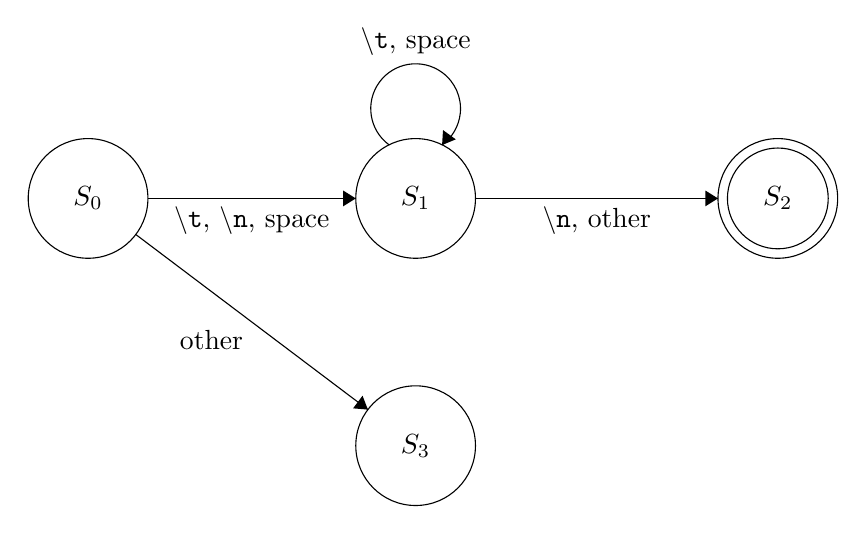
\begin{tikzpicture}[scale=0.2]
\tikzstyle{every node}+=[inner sep=0pt]
\draw [black] (4,-10.9) circle (3.8);
\draw (4,-10.9) node {$S_0$};
\draw [black] (24.8,-10.9) circle (3.8);
\draw (24.8,-10.9) node {$S_1$};
\draw [black] (47.8,-10.9) circle (3.8);
\draw (47.8,-10.9) node {$S_2$};
\draw [black] (47.8,-10.9) circle (3.2);
\draw [black] (24.8,-26.6) circle (3.8);
\draw (24.8,-26.6) node {$S_3$};
\draw [black] (7.8,-10.9) -- (21,-10.9);
\fill [black] (21,-10.9) -- (20.2,-10.4) -- (20.2,-11.4);
\draw (14.4,-11.4) node [below] {\texttt{\textbackslash t},\ \texttt{\textbackslash n},\ space};
\draw [black] (28.6,-10.9) -- (44,-10.9);
\fill [black] (44,-10.9) -- (43.2,-10.4) -- (43.2,-11.4);
\draw (36.3,-11.4) node [below] {\texttt{\textbackslash n},\ other};
\draw [black] (23.125,-7.506) arc (234:-54:2.85);
\draw (24.8,-1.85) node [above] {\texttt{\textbackslash t},\ space};
\fill [black] (26.48,-7.51) -- (27.35,-7.15) -- (26.54,-6.56);
\draw [black] (7.03,-13.19) -- (21.77,-24.31);
\fill [black] (21.77,-24.31) -- (21.43,-23.43) -- (20.83,-24.23);
\draw (11.84,-19.25) node [below] {other};
\end{tikzpicture}
\end{center}

\subsection{Detailed Explanation}

The is_space function in a lexical analyzer checks whether a part of the source code consists of whitespace characters like spaces, tabs, or newlines. It scans the input line character by character using a state machine approach. If it encounters whitespace, it transitions through states, eventually returning a token indicating that whitespace has been found. If the characters are not whitespace, it flags them as invalid. This process is crucial in a lexical analyzer for properly separating tokens in the source code.


\section{Comments}



\subsection{Automata}

\begin{center}
\begin{tikzpicture}[scale=0.2]
\tikzstyle{every node}+=[inner sep=0pt]
\draw [black] (4,-10.9) circle (3.8);
\draw (4,-10.9) node {$S_0$};
\draw [black] (19.9,-10.9) circle (3.8);
\draw (19.9,-10.9) node {$S_1$};
\draw [black] (35.8,-10.9) circle (3.8);
\draw (35.8,-10.9) node {$S_2$};
\draw [black] (51.2,-10.9) circle (3.8);
\draw (51.2,-10.9) node {$S_3$};
\draw [black] (19.9,-26.3) circle (3.8);
\draw (19.9,-26.3) node {$S_4$};
\draw [black] (7.8,-10.9) -- (16.1,-10.9);
\fill [black] (16.1,-10.9) -- (15.3,-10.4) -- (15.3,-11.4);
\draw (11.95,-11.4) node [below] {$/$};
\draw [black] (23.7,-10.9) -- (32,-10.9);
\fill [black] (32,-10.9) -- (31.2,-10.4) -- (31.2,-11.4);
\draw (27.85,-11.4) node [below] {$/$};
\draw [black] (39.6,-10.9) -- (47.4,-10.9);
\fill [black] (47.4,-10.9) -- (46.6,-10.4) -- (46.6,-11.4);
\draw (43.5,-11.4) node [below] {\texttt{\textbackslash n}};
\draw [black] (6.73,-13.54) -- (17.17,-23.66);
\fill [black] (17.17,-23.66) -- (16.94,-22.74) -- (16.25,-23.46);
\draw (9.38,-19.08) node [below] {$other$};
\draw [black] (19.9,-14.7) -- (19.9,-22.5);
\fill [black] (19.9,-22.5) -- (20.4,-21.7) -- (19.4,-21.7);
\draw (19.4,-18.6) node [left] {$other$};
\draw [black] (34.125,-7.506) arc (234:-54:2.85);
\draw (35.8,-1.85) node [above] {$other,\mbox{ }/$};
\fill [black] (37.48,-7.51) -- (38.35,-7.15) -- (37.54,-6.56);
\end{tikzpicture}
\end{center}

\subsection{Detailed Explanation}

The is_comment function in a lexical analyzer is responsible for detecting comments in a line of code, typically for single-line comments. It checks if a part of the source code starts with a comment indicator (//), and if so, captures the content of the comment until the end of the line or an invalid sequence is encountered. The function uses a state machine approach to handle different stages of comment detection: it starts by checking for the initial comment markers (//), then captures the content inside the comment, and finally returns a token representing the comment. If an invalid sequence is encountered (e.g., characters not following the expected comment format), the function returns an "invalid" token. This is an essential part of the lexical analysis process for ignoring comments while parsing the code.


\section{Operators}

\subsection{Automata}

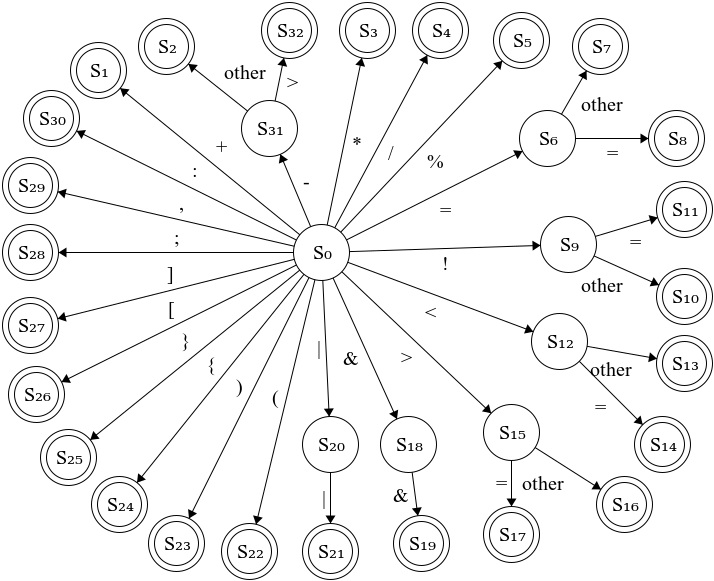
\includegraphics[width=0.9\textwidth]{images/ops.png}

\subsection{Detailed Explanation}

The \texttt{is\_operator} function in a lexical analyzer is responsible for detecting and categorizing operators and punctuation marks in a line of code. This function uses a state machine approach to handle the detection of various operators, including arithmetic operators (e.g., \( + \), \( - \), \( * \)), relational operators (e.g., \( == \), \( < \), \( \geq \)), logical operators (e.g., \( \&\& \), \( || \)), and other symbols (e.g., parentheses, semicolons, and commas). The function scans the line character by character, transitioning between states as it encounters known operator symbols. If it identifies a valid operator or symbol, it returns a corresponding token (such as \texttt{T\_AOp\_AD} for addition, \texttt{T\_ROp\_E} for equality check, or \texttt{T\_Semicolon} for semicolon). If an unrecognized character is encountered, the function returns an ``Invalid'' token, signaling an error. This function plays a critical role in the lexical analysis phase of a compiler, where operators and punctuation are identified and classified for further processing.



\section{HexaDecimal}


\subsection{Automata}

\begin{center}
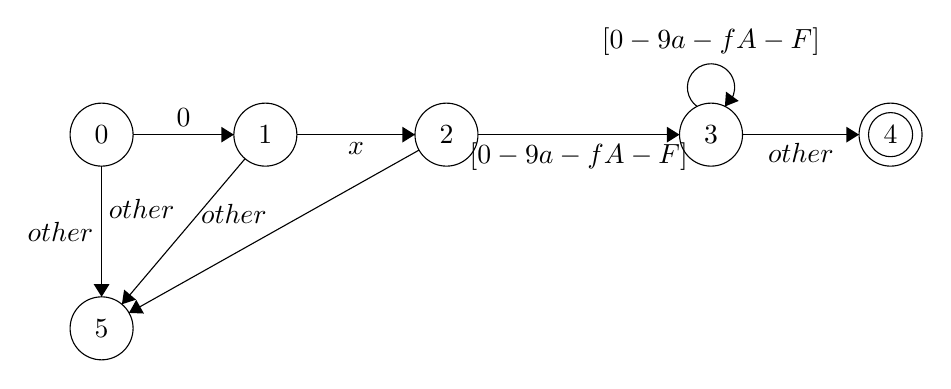
\begin{tikzpicture}[scale=0.2]
\tikzstyle{every node}+=[inner sep=0pt]
\draw [black] (4.8,-6.9) circle (2);
\draw (4.8,-6.9) node {$0$};
\draw [black] (15.2,-6.9) circle (2);
\draw (15.2,-6.9) node {$1$};
\draw [black] (26.7,-6.9) circle (2);
\draw (26.7,-6.9) node {$2$};
\draw [black] (4.8,-19.2) circle (2);
\draw (4.8,-19.2) node {$5$};
\draw [black] (43.5,-6.9) circle (2);
\draw (43.5,-6.9) node {$3$};
\draw [black] (54.9,-6.9) circle (2);
\draw (54.9,-6.9) node {$4$};
\draw [black] (54.9,-6.9) circle (1.4);
\draw [black] (6.8,-6.9) -- (13.2,-6.9);
\fill [black] (13.2,-6.9) -- (12.4,-6.4) -- (12.4,-7.4);
\draw (10,-6.4) node [above] {$0$};
\draw [black] (4.8,-8.9) -- (4.8,-17.2);
\fill [black] (4.8,-17.2) -- (5.3,-16.4) -- (4.3,-16.4);
\draw (4.3,-13.05) node [left] {$other$};
\draw [black] (17.2,-6.9) -- (24.7,-6.9);
\fill [black] (24.7,-6.9) -- (23.9,-6.4) -- (23.9,-7.4);
\draw (20.95,-7.4) node [below] {$x$};
\draw [black] (28.7,-6.9) -- (41.5,-6.9);
\fill [black] (41.5,-6.9) -- (40.7,-6.4) -- (40.7,-7.4);
\draw (35.1,-7.4) node [below] {$[0-9a-fA-F]$};
\draw [black] (42.618,-5.114) arc (234:-54:1.5);
\draw (43.5,-1.9) node [above] {$[0-9a-fA-F]$};
\fill [black] (44.38,-5.11) -- (45.26,-4.76) -- (44.45,-4.17);
\draw [black] (45.5,-6.9) -- (52.9,-6.9);
\fill [black] (52.9,-6.9) -- (52.1,-6.4) -- (52.1,-7.4);
\draw (49.2,-7.4) node [below] {$other$};
\draw [black] (13.91,-8.43) -- (6.09,-17.67);
\fill [black] (6.09,-17.67) -- (6.99,-17.38) -- (6.23,-16.74);
\draw (9.45,-11.61) node [left] {$other$};
\draw [black] (24.96,-7.88) -- (6.54,-18.22);
\fill [black] (6.54,-18.22) -- (7.49,-18.26) -- (7,-17.39);
\draw (13.2,-12.55) node [above] {$other$};
\end{tikzpicture}
\end{center}

\subsection{Detailed Explanation}
The \texttt{is\_hexadecimal} function implements a five-state DFA for strict hexadecimal number validation. State 0 requires a leading '0', transitioning to state 1 which demands either 'x' or 'X'. State 2 then requires at least one hexadecimal digit (0-9, a-f, A-F), with state 3 consuming subsequent hexadecimal digits. The final state (state 4) validates that proper hexadecimal digits follow the prefix before returning a \texttt{T\_Hexadecimal} token.

This implementation enforces the language specification that hexadecimal literals must have at least one digit after the prefix. The function uses \texttt{isxdigit()} for proper character classification and preserves the original casing of hexadecimal digits in the token content. Invalid sequences like "0x" without subsequent digits are properly rejected with \texttt{Invalid} tokens.

\section{Decimal}


\subsection{Automata}

\begin{center}
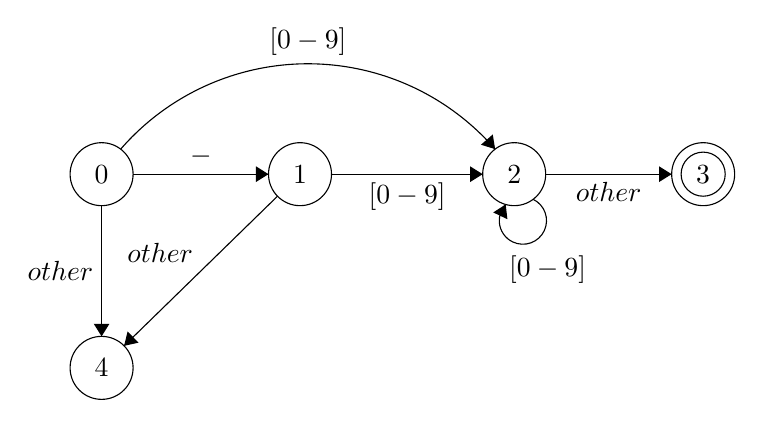
\begin{tikzpicture}[scale=0.2]
\tikzstyle{every node}+=[inner sep=0pt]
\draw [black] (4.8,-9.4) circle (2);
\draw (4.8,-9.4) node {$0$};
\draw [black] (17.4,-9.4) circle (2);
\draw (17.4,-9.4) node {$1$};
\draw [black] (31,-9.4) circle (2);
\draw (31,-9.4) node {$2$};
\draw [black] (4.8,-21.7) circle (2);
\draw (4.8,-21.7) node {$4$};
\draw [black] (43,-9.4) circle (2);
\draw (43,-9.4) node {$3$};
\draw [black] (43,-9.4) circle (1.4);
\draw [black] (6.8,-9.4) -- (15.4,-9.4);
\fill [black] (15.4,-9.4) -- (14.6,-8.9) -- (14.6,-9.9);
\draw (11.1,-8.9) node [above] {$-$};
\draw [black] (4.8,-11.4) -- (4.8,-19.7);
\fill [black] (4.8,-19.7) -- (5.3,-18.9) -- (4.3,-18.9);
\draw (4.3,-15.55) node [left] {$other$};
\draw [black] (33,-9.4) -- (41,-9.4);
\fill [black] (41,-9.4) -- (40.2,-8.9) -- (40.2,-9.9);
\draw (37,-9.9) node [below] {$other$};
\draw [black] (6.012,-7.811) arc (139.02995:40.97005:15.745);
\fill [black] (29.79,-7.81) -- (29.64,-6.88) -- (28.89,-7.53);
\draw (17.9,-1.89) node [above] {$[0-9]$};
\draw [black] (19.4,-9.4) -- (29,-9.4);
\fill [black] (29,-9.4) -- (28.2,-8.9) -- (28.2,-9.9);
\draw (24.2,-9.9) node [below] {$[0-9]$};
\draw [black] (15.97,-10.8) -- (6.23,-20.3);
\fill [black] (6.23,-20.3) -- (7.15,-20.1) -- (6.45,-19.39);
\draw (8.52,-15.07) node [above] {$other$};
\draw [black] (32.196,-10.993) arc (64.61966:-223.38034:1.5);
\draw (33.12,-14.55) node [below] {$[0-9]$};
\fill [black] (30.46,-11.32) -- (29.67,-11.83) -- (30.57,-12.26);
\end{tikzpicture}
\end{center}

\subsection{Detailed Explanation}
The \texttt{is\_decimal} function implements a four-state DFA for recognizing both positive and negative decimal integers. State 0 handles the optional minus sign, transitioning to state 1 if present. State 2 requires at least one digit (0-9) and continues consuming digits until a non-digit character is encountered. The final state (state 3) validates that at least one digit was collected before returning a \texttt{T\_Decimal} token.

This implementation properly handles edge cases like standalone minus signs (invalid) and maximum number length constraints. The function also preserves the original string representation of the number (including leading zeros) in the token content for accurate source representation. Number validation occurs without conversion to numeric values, maintaining precision during lexical analysis.

\section{Keywords}

\subsection{Automata}

\begin{center}
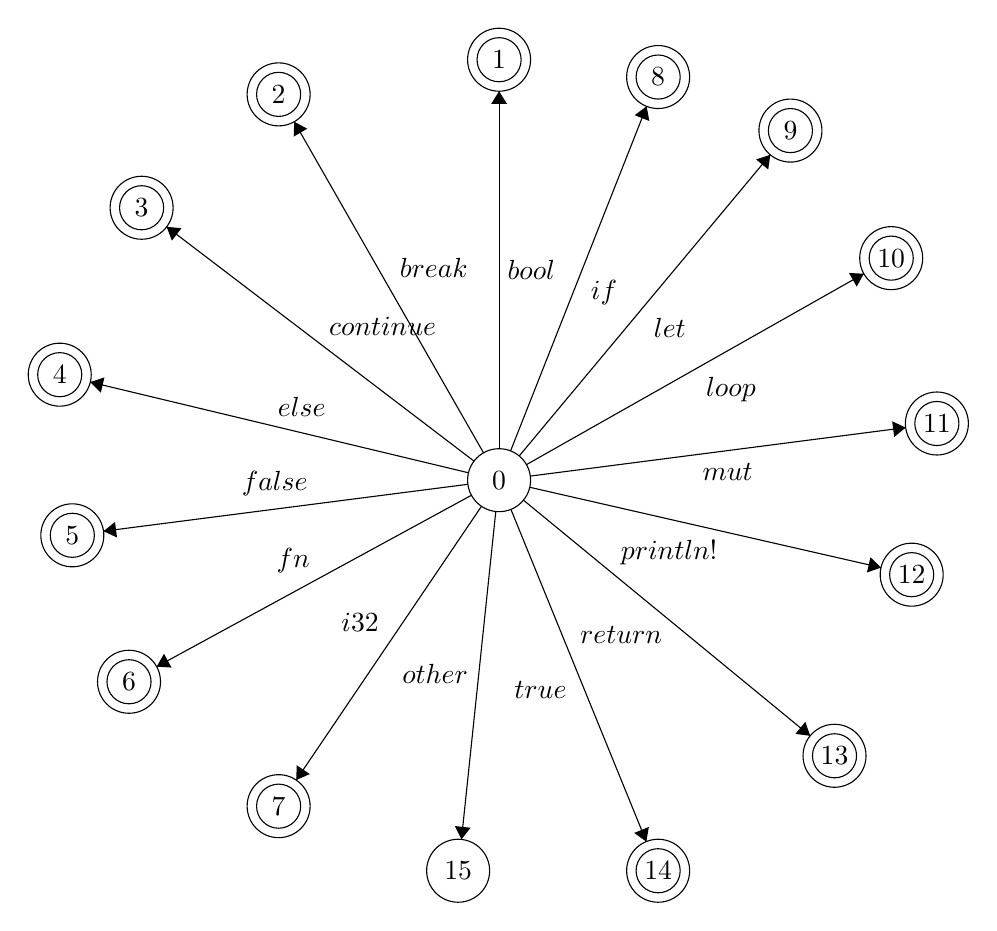
\begin{tikzpicture}[scale=0.2]
\tikzstyle{every node}+=[inner sep=0pt]
\draw [black] (30.1,-28.7) circle (2);
\draw (30.1,-28.7) node {$0$};
\draw [black] (30.1,-2) circle (2);
\draw (30.1,-2) node {$1$};
\draw [black] (30.1,-2) circle (1.4);
\draw [black] (16.1,-4.2) circle (2);
\draw (16.1,-4.2) node {$2$};
\draw [black] (16.1,-4.2) circle (1.4);
\draw [black] (7.4,-11.4) circle (2);
\draw (7.4,-11.4) node {$3$};
\draw [black] (7.4,-11.4) circle (1.4);
\draw [black] (2.2,-22) circle (2);
\draw (2.2,-22) node {$4$};
\draw [black] (2.2,-22) circle (1.4);
\draw [black] (3,-32.2) circle (2);
\draw (3,-32.2) node {$5$};
\draw [black] (3,-32.2) circle (1.4);
\draw [black] (6.6,-41.5) circle (2);
\draw (6.6,-41.5) node {$6$};
\draw [black] (6.6,-41.5) circle (1.4);
\draw [black] (16.1,-49.4) circle (2);
\draw (16.1,-49.4) node {$7$};
\draw [black] (16.1,-49.4) circle (1.4);
\draw [black] (27.5,-53.5) circle (2);
\draw (27.5,-53.5) node {$15$};
\draw [black] (40.2,-3.1) circle (2);
\draw (40.2,-3.1) node {$8$};
\draw [black] (40.2,-3.1) circle (1.4);
\draw [black] (48.6,-6.5) circle (2);
\draw (48.6,-6.5) node {$9$};
\draw [black] (48.6,-6.5) circle (1.4);
\draw [black] (55,-14.6) circle (2);
\draw (55,-14.6) node {$10$};
\draw [black] (55,-14.6) circle (1.4);
\draw [black] (57.9,-25.1) circle (2);
\draw (57.9,-25.1) node {$11$};
\draw [black] (57.9,-25.1) circle (1.4);
\draw [black] (56.3,-34.7) circle (2);
\draw (56.3,-34.7) node {$12$};
\draw [black] (56.3,-34.7) circle (1.4);
\draw [black] (51.4,-46.2) circle (2);
\draw (51.4,-46.2) node {$13$};
\draw [black] (51.4,-46.2) circle (1.4);
\draw [black] (40.2,-53.5) circle (2);
\draw (40.2,-53.5) node {$14$};
\draw [black] (40.2,-53.5) circle (1.4);
\draw [black] (30.1,-26.7) -- (30.1,-4);
\fill [black] (30.1,-4) -- (29.6,-4.8) -- (30.6,-4.8);
\draw (30.6,-15.35) node [right] {$bool$};
\draw [black] (29.11,-26.96) -- (17.09,-5.94);
\fill [black] (17.09,-5.94) -- (17.06,-6.88) -- (17.92,-6.38);
\draw (23.76,-15.23) node [right] {$break$};
\draw [black] (28.51,-27.49) -- (8.99,-12.61);
\fill [black] (8.99,-12.61) -- (9.32,-13.49) -- (9.93,-12.7);
\draw (22.7,-19.55) node [above] {$continue$};
\draw [black] (28.16,-28.23) -- (4.14,-22.47);
\fill [black] (4.14,-22.47) -- (4.81,-23.14) -- (5.04,-22.17);
\draw (17.57,-24.7) node [above] {$else$};
\draw [black] (28.12,-28.96) -- (4.98,-31.94);
\fill [black] (4.98,-31.94) -- (5.84,-32.34) -- (5.71,-31.35);
\draw (15.85,-29.73) node [above] {$false$};
\draw [black] (28.34,-29.66) -- (8.36,-40.54);
\fill [black] (8.36,-40.54) -- (9.3,-40.6) -- (8.82,-39.72);
\draw (17.02,-34.6) node [above] {$fn$};
\draw [black] (28.98,-30.36) -- (17.22,-47.74);
\fill [black] (17.22,-47.74) -- (18.08,-47.36) -- (17.25,-46.8);
\draw (22.49,-37.71) node [left] {$i32$};
\draw [black] (30.83,-26.84) -- (39.47,-4.96);
\fill [black] (39.47,-4.96) -- (38.71,-5.52) -- (39.64,-5.89);
\draw (35.9,-16.77) node [right] {$if$};
\draw [black] (31.38,-27.16) -- (47.32,-8.04);
\fill [black] (47.32,-8.04) -- (46.42,-8.33) -- (47.19,-8.97);
\draw (39.9,-19.04) node [right] {$let$};
\draw [black] (31.84,-27.71) -- (53.26,-15.59);
\fill [black] (53.26,-15.59) -- (52.32,-15.54) -- (52.81,-16.41);
\draw (44.82,-22.15) node [below] {$loop$};
\draw [black] (32.08,-28.44) -- (55.92,-25.36);
\fill [black] (55.92,-25.36) -- (55.06,-24.96) -- (55.19,-25.96);
\draw (44.61,-27.59) node [below] {$mut$};
\draw [black] (32.05,-29.15) -- (54.35,-34.25);
\fill [black] (54.35,-34.25) -- (53.68,-33.59) -- (53.46,-34.56);
\draw (40.9,-32.47) node [below] {$println!$};
\draw [black] (31.65,-29.97) -- (49.85,-44.93);
\fill [black] (49.85,-44.93) -- (49.55,-44.04) -- (48.92,-44.81);
\draw (37.85,-37.94) node [below] {$return$};
\draw [black] (30.85,-30.55) -- (39.45,-51.65);
\fill [black] (39.45,-51.65) -- (39.61,-50.72) -- (38.68,-51.1);
\draw (34.41,-42) node [left] {$true$};
\draw [black] (29.89,-30.69) -- (27.71,-51.51);
\fill [black] (27.71,-51.51) -- (28.29,-50.77) -- (27.29,-50.66);
\draw (28.15,-41) node [left] {$other$};
\end{tikzpicture}
\end{center}

\subsection{Detailed Explanation}
The \texttt{is\_keyword} function implements a deterministic finite automaton (DFA) that recognizes the 14 reserved keywords of the Trust language. Each keyword is treated as a fixed literal pattern that must match exactly, with case sensitivity. The function first checks for the longest possible keyword match ("println!") before proceeding to shorter ones to ensure correct tokenization. After finding a potential match, it verifies that the match isn't part of a larger identifier by checking the following character isn't a letter, digit, or underscore. This strict validation prevents keywords from being misidentified within identifiers while maintaining language semantics.

The implementation uses a state machine that transitions through each character of potential keywords, with failure paths that efficiently fall back to identifier recognition when no keyword matches. This approach provides O(n) time complexity where n is the length of the longest keyword, making it highly efficient for lexical analysis.


\section{Strings}

\subsection{Automata}

\begin{center}
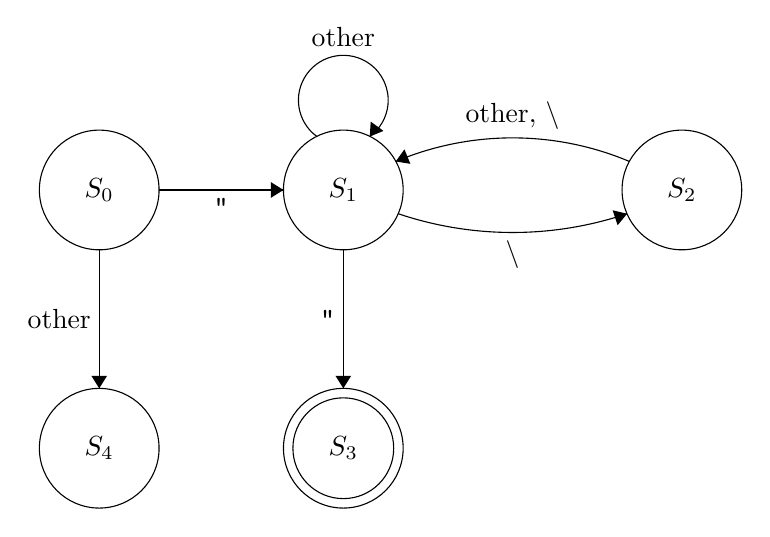
\begin{tikzpicture}[scale=0.2]
\tikzstyle{every node}+=[inner sep=0pt]
\draw [black] (4.7,-10.9) circle (3.8);
\draw (4.7,-10.9) node {$S_0$};
\draw [black] (20.2,-10.9) circle (3.8);
\draw (20.2,-10.9) node {$S_1$};
\draw [black] (41.7,-10.9) circle (3.8);
\draw (41.7,-10.9) node {$S_2$};
\draw [black] (20.2,-27.3) circle (3.8);
\draw (20.2,-27.3) node {$S_3$};
\draw [black] (20.2,-27.3) circle (3.2);
\draw [black] (4.7,-27.3) circle (3.8);
\draw (4.7,-27.3) node {$S_4$};
\draw [black] (8.5,-10.9) -- (16.4,-10.9);
\fill [black] (16.4,-10.9) -- (15.6,-10.4) -- (15.6,-11.4);
\draw (12.45,-11.4) node [below] {\texttt{"}};
\draw [black] (4.7,-14.7) -- (4.7,-23.5);
\fill [black] (4.7,-23.5) -- (5.2,-22.7) -- (4.2,-22.7);
\draw (4.2,-19.1) node [left] {other};
\draw [black] (18.525,-7.506) arc (234:-54:2.85);
\draw (20.2,-1.85) node [above] {other};
\fill [black] (21.88,-7.51) -- (22.75,-7.15) -- (21.94,-6.56);
\draw [black] (38.217,-12.408) arc (-71.36814:-108.63186:22.746);
\fill [black] (38.22,-12.41) -- (37.3,-12.19) -- (37.62,-13.14);
\draw (30.95,-14.1) node [below] {\texttt{\textbackslash}};
\draw [black] (20.2,-14.7) -- (20.2,-23.5);
\fill [black] (20.2,-23.5) -- (20.7,-22.7) -- (19.7,-22.7);
\draw (19.7,-19.1) node [left] {\texttt{"}};
\draw [black] (23.533,-9.089) arc (112.82624:67.17376:19.118);
\fill [black] (23.53,-9.09) -- (24.46,-9.24) -- (24.08,-8.32);
\draw (30.95,-7.09) node [above] {other, \texttt{\textbackslash}};
\end{tikzpicture}
\end{center}

\subsection{Detailed Explanation}

The is_string function in a lexical analyzer is designed to detect and process string literals in the source code. It scans a line character by character, looking for strings enclosed in double quotes ("). The function handles different scenarios, such as escape sequences (\") and the correct closing of the string literal. Using a state machine, it transitions through various states: it starts by detecting the opening quote, then handles escape characters, and finally detects the closing quote to complete the string. If the string is valid, it returns a token of type T_String containing the string content. If an invalid string is encountered (e.g., the string is incomplete or malformed), it returns an Invalid token. This function is a key part of the lexical analysis process, ensuring strings are correctly identified and tokenized for further processing.


\section{IDs}


\subsection{Automata}

\begin{center}
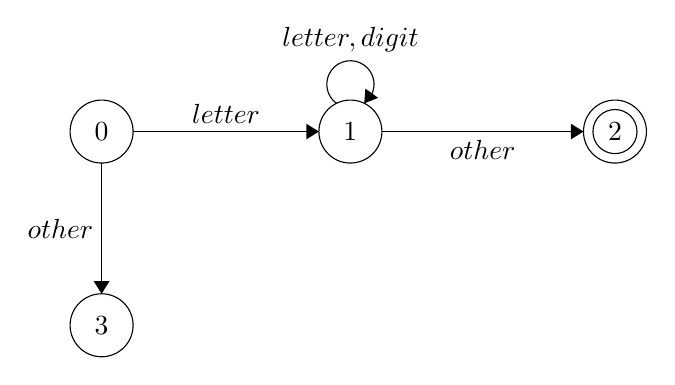
\begin{tikzpicture}[scale=0.2]
\tikzstyle{every node}+=[inner sep=0pt]
\draw [black] (4.8,-6.9) circle (2);
\draw (4.8,-6.9) node {$0$};
\draw [black] (20.6,-6.9) circle (2);
\draw (20.6,-6.9) node {$1$};
\draw [black] (37.4,-6.9) circle (2);
\draw (37.4,-6.9) node {$2$};
\draw [black] (37.4,-6.9) circle (1.4);
\draw [black] (4.8,-19.2) circle (2);
\draw (4.8,-19.2) node {$3$};
\draw [black] (6.8,-6.9) -- (18.6,-6.9);
\fill [black] (18.6,-6.9) -- (17.8,-6.4) -- (17.8,-7.4);
\draw (12.7,-6.4) node [above] {$letter$};
\draw [black] (4.8,-8.9) -- (4.8,-17.2);
\fill [black] (4.8,-17.2) -- (5.3,-16.4) -- (4.3,-16.4);
\draw (4.3,-13.05) node [left] {$other$};
\draw [black] (22.6,-6.9) -- (35.4,-6.9);
\fill [black] (35.4,-6.9) -- (34.6,-6.4) -- (34.6,-7.4);
\draw (29,-7.4) node [below] {$other$};
\draw [black] (19.718,-5.114) arc (234:-54:1.5);
\draw (20.6,-1.9) node [above] {$letter,digit$};
\fill [black] (21.48,-5.11) -- (22.36,-4.76) -- (21.55,-4.17);
\end{tikzpicture}
\end{center}

\subsection{Detailed Explanation}
The \texttt{is\_id} function implements the identifier recognition grammar through a three-state DFA. The initial state requires the first character to be either an underscore or letter (state 1). Subsequent characters transition to state 2 where letters, digits, or underscores are accepted. The function continues consuming characters until encountering a non-matching character, at which point it verifies the collected identifier doesn't match any keyword (using \texttt{is\_keyword}) before returning a \texttt{T\_Id} token.

This implementation carefully handles Unicode characters by using \texttt{isalpha()} and \texttt{isalnum()} functions for proper character classification. The function also maintains position information to support precise error reporting when invalid identifiers are encountered. The lookahead verification ensures identifiers don't conflict with language keywords while allowing maximum flexibility in naming conventions.


\end{document}
